% proposal.tex
\documentclass[main.tex]{subfiles}
\begin{document}
\chapter{Proposed Work} \label{ch:proposal}

The use of AM technologies to produce small batches of highly customized, complex parts, in a reduced development cycle results extremely attractive. While constructing failure envelopes can help overcome the wariness of industrial segments to design end-user parts, this resource is still not easy to implement, requiring a large number of mechanical tests and specialized equipment to properly map the failure behavior of a particular material. Additional complexity stems from what was shown in Section \ref{sec:SSICAM}: processing the same material under related AM technologies yields completely different failure envelopes, implying that no generalizations should be made, and each material-process pairing needs to be studied on a case-by-case basis. In general, for AM parts to be adopted, engineers have to be able to confidently assess the probability of part failure under particular loading conditions, predict the expected mechanical properties of AM parts, and understand the underlying physics of the process. None of these considerations are completely understood at the time of this work. The solutions presented in this proposal are aimed at solving one of these three issues. This work aims to provide the tools required to understand and predict properties and mechanical performance of parts manufactured through FFF. Some, if not all of the procedures developed in this work could even be extrapolated to other AM techniques. The end goal is having the framework necessary to streamline the development of failure envelopes for FFF as much as possible, making a compelling case for adoption of this technology in the production of end user parts subjected to complex loading conditions. 

\section{Objectives} \label{sec:objectives}

The set of printing conditions that lead to an optimal part in terms of mechanical properties aren't still fully comprehended. However, if there existed an FFF machine with in-line sensors that allowed monitoring a variety of process-variables, as well as data generated from mechanical tests and ancillary experiments, this would constitute an interesting case for development of a Machine Learning (ML) system. These excel in cases where the inputs and outcomes of a particular phenomena or task are known, but connecting the two through an explicit set of rules or relationships can result extremely complex and time consuming \cite{Chollet2018}. In this manner, ML models are \emph{trained}, as opposed to explicitly programmed. Figure \ref{fig:MLvsP} compares the differences between ML and traditional programming philosophies. 

\begin{figure}[!htbp]
	\center
	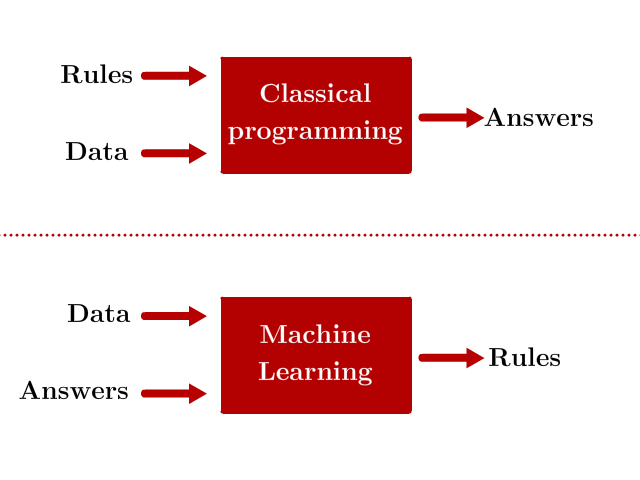
\includegraphics[height=6.5cm]{ML}
	\caption{Differences between traditional programming and machine learning. \cite{Chollet2018}} \label{fig:MLvsP}
\end{figure}

The fundamental goal of this research is to predict FFF part mechanical performance by finding clear relations between processing and strength through the use of sensors and machine learning. The success of this project would allow design engineers to confidently assess if a part manufactured through FFF will meet the mechanical requirements imposed by its intended application. This work proposes developing and using a modified printer with force and print speed sensors, as well as mechanical testing and $\mu$CT scans to generate data that can be used to train a predictive tool based on ML. This tool can then be used to predict final mechanical properties of the part based on the data generated during the print. This ML system would accept filament dimensions, printing temperature, filament force, filament velocity, print orientation, or any subset of these items as inputs, and produce final part porosity and mechanical strength in a particular load direction as outputs. The specifics of the architecture of the ML system are  still under development, as it may prove useful to segment the problem into several sub-systems connected in series, in what is called a machine learning \emph{pipeline} \cite{Geron2019}. However, given the specifics of the task, one can conclude that the system will involve supervised learning applied to a regression problem, given that all the inputs to the system will consist of pre-selected attributes, and the mechanical response and/or porosity of a printed part can be treated as a target value the ML system has to be able to predict. 

\section{Preliminary results} \label{sec:prelim}


\begin{figure}[!htbp]
	\center
	\includegraphics[height=10cm]{forcesetup}
	\caption{Schematic of modified FFF printer with sensors} \label{fig:shakira}
\end{figure}

\begin{figure}[!htbp]
	\center
	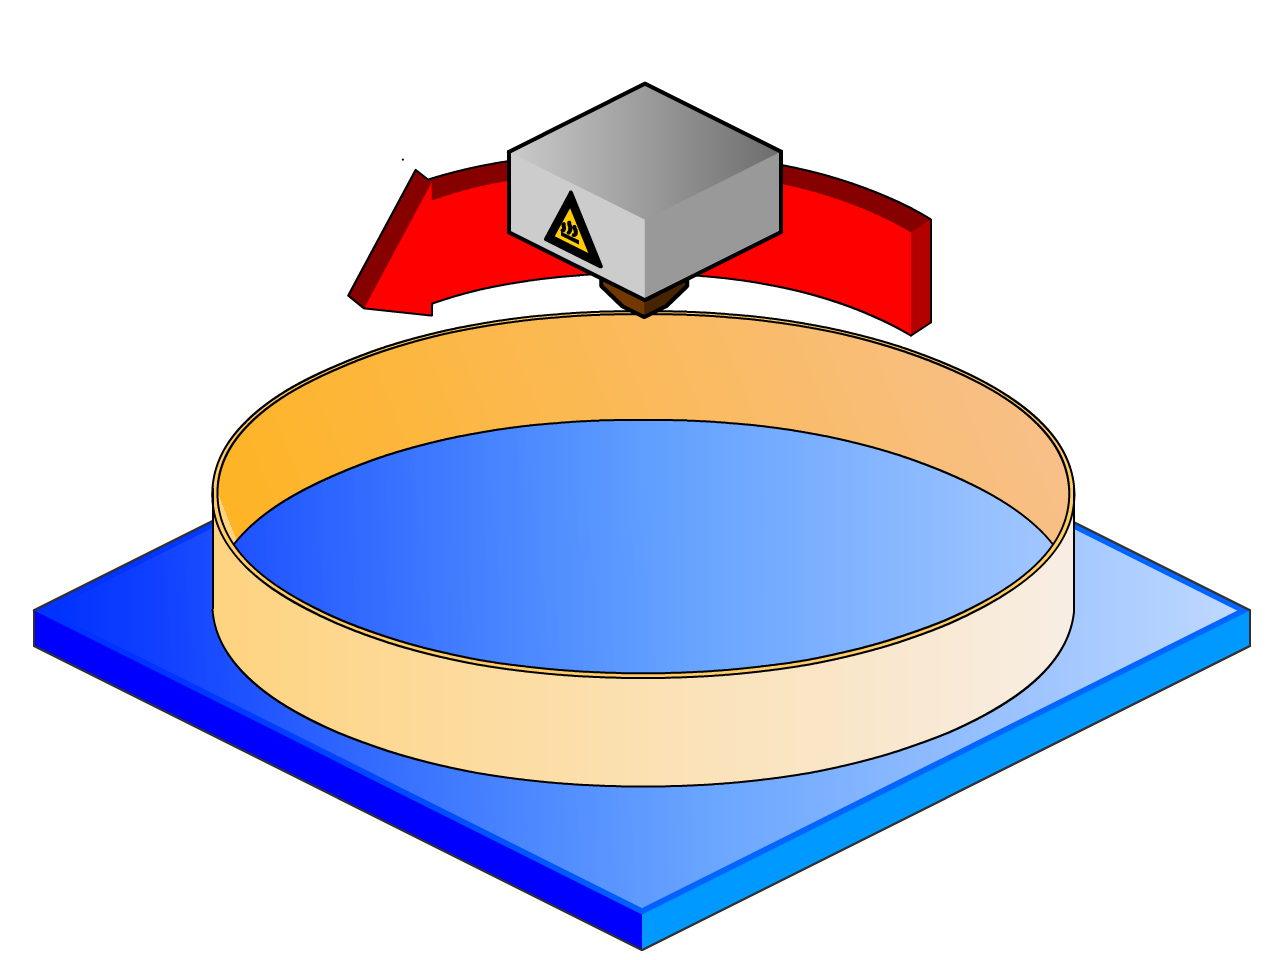
\includegraphics[width=0.8\linewidth]{cyl_shakira}
	\caption{Continuous print for force-velocity data collection} \label{fig:cyl}
\end{figure}

\begin{figure}[!htbp]
	\center
	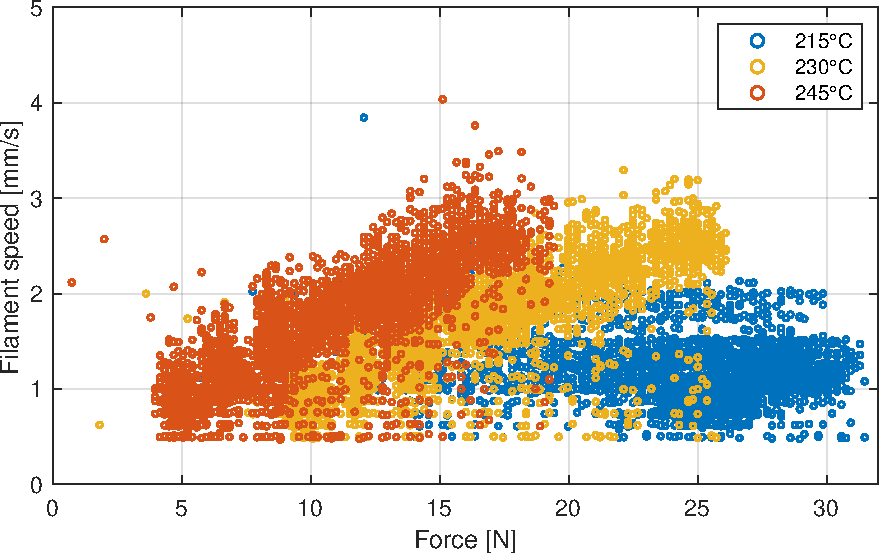
\includegraphics[width=0.8\linewidth]{ABS_prelim.pdf}
	\caption{Comparison of Force requirements for ABS} \label{fig:absprelim}
\end{figure}

\section{Future work} \label{sec:fw}



%__________________________________________________________________________________________________________
% Nomenclature introduced in this chapter:
\nomenclature[A]{ML}{Machine Learning}% 

% Symbols introduced in this chapter:
\nomenclature[S]{$X_t$}{Tensile strength in the 1-1 direction \nomunit{$MPa$}}
\end{document}